\documentclass[12pt]{article}
\usepackage{hyperref}
\usepackage{graphicx}
\begin{document}
{\LARGE \textbf Short Answer}

1. We use EWs to compare the relative strengths of different lines in a spectrum (or the same line in different spectrums) because the continuum intensity varies. The flux value is divided by the continuum and therefore shows the fraction of light (and not the actual number of photons) absorbed by the medium between the telescope and the star. This is independent of resolution and allows for low-resolution sources to be used, but information like the skew or shape of the peaks is lost. Ratios of EW can be used to calibrate for temperatures.

2. These H-$\alpha$, H-$\beta$ lines etc. are the result of emission/absorption from electrons transitioning between different energy levels of the hydrogen atom. As stars are predominantly made up of hydrogen, we use the existence of the hydrogen spectral lines to verify if the spectrum is from a star.

3. The strength of the lines is related to the surface temperature of the star. The same star at different temperatures will record a different wavelength for the location of the peak, as well as different flux (and so different EW) values. The surface temperature can be dohetermined by Wien's law, i.e.
T = $ \frac{2.9*10^7}{\lambda_{peak}} $. Furthermore, in general, denser stars have thinner peaks due to the smaller number of collisions that happen. The effect of temperature on the EW is still dominant, however. Also, the strength of a line is proportional to the relative abundance of that element inside the star.

4. Other absorption lines: \\
\includegraphics[width=15cm]{../otherpeaks}\\
Fig 1. Alternative peaks - on the left, I have identified peaks at 3836$\AA$ (H-eta), 3890$\AA$ (He-I), 3934$\AA$ (K) and 3970$\AA$ (H), where H and K are Ionized Calcium.   On the right, we have a peak at 5582$\AA$ (not certain, but I believe this is Titanium Oxide) and at 6306$\AA$ (O-I). I used this source from UChicago to identify the emission lines: \url{http://astro.uchicago.edu/~subbarao/newWeb/line.html}\\
\includegraphics[width=12cm]{../otherpeakszoom}\\
Fig 2. This is a zoomed-in version of Fig. 1, to see the peaks at the lower wavelengths more clearly.\\
\includegraphics[width=12cm]{../anotherpeaks}\\
Fig 3. This is another spectra to show the same peaks appearing for another star.\\


{\LARGE \textbf Other Work} \\
\textbf {1. Using the sqlcl.py module within Python to query the SDSS database (DR9).}
- This seeks for the standard (calibration) stars as defined on SDSS's "Algorithms" webpage: \url{http://www.sdss3.org/dr9/algorithms/boss_std_ts.php}. \\
- There is one modification: instead of \\ $\sqrt{((u-g)-0.82)^2+((g-r)-0.3)^2+((r-i)-0.09)^2+((i-z)-0.02)^2}<0.08$ we used $|(u-g)-0.82|<0.08$, $|(g-r)-0.3|<0.08$ etc. \\
- The output gives the extinction (in the g-band), the recorded flux, equivalent width and continuum values given in galSpecLine for the H-$\alpha$, H-$\beta$, H-$\gamma$, H-$\delta$ lines. \\
- However, due to the reported equivalent widths being unreasonable compared to manual estimations, the query also extracts the plate-mjd-fiber values and downloads, via wget, the relevant FITS file for this plate-mjd-fiber combination. \\
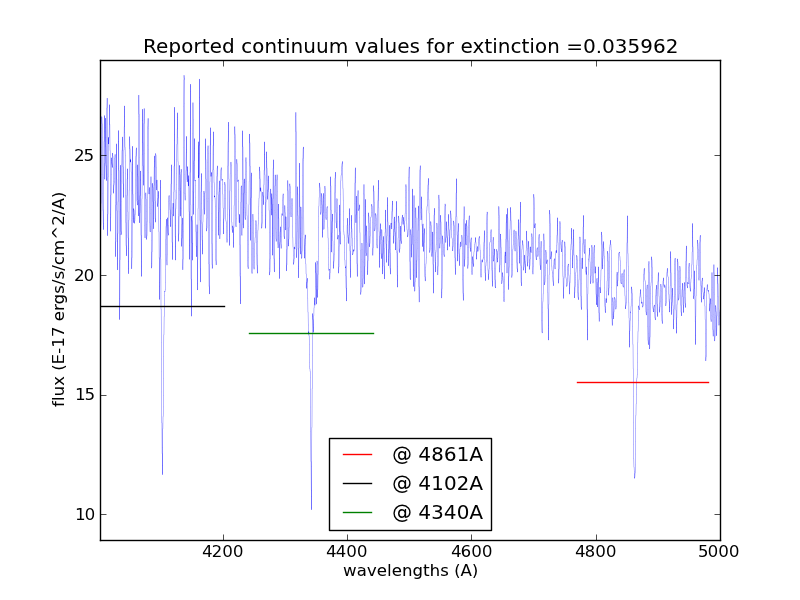
\includegraphics[width=6cm]{../035}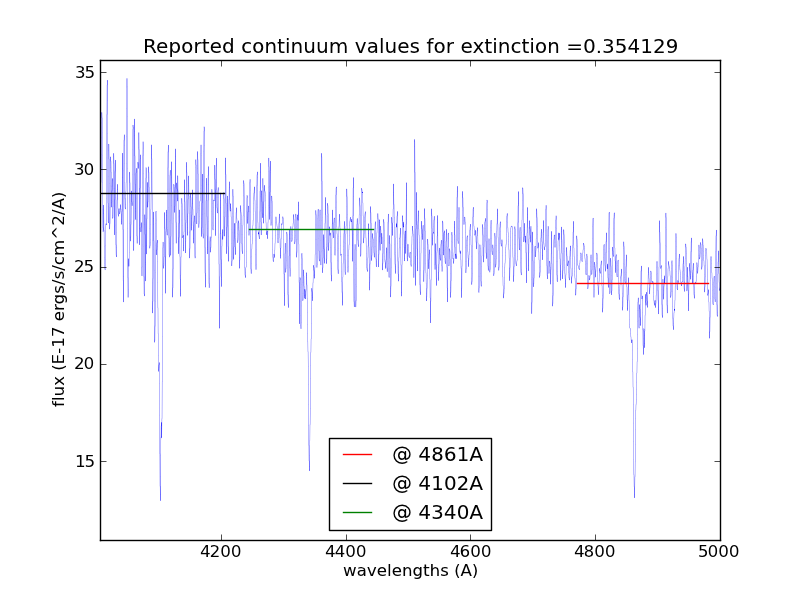
\includegraphics[width=6cm]{../355}\\
Fig 4. The recorded continuum values in GalSpecLine seem to be only valid for high (above 0.25) extinction values.\\
\textbf{2. Generating the new continuum, flux and equivalent width values}\\
- The spectra are first corrected for redshift using the redshift value from HDU 2 (copy of specObj table from SDSS).\\
- A cubic spline is used to smooth the spectrum. To plot the spline, I use a step size one-tenth of the step size of the wavelengths in the FITS file. \\
- Near the location of each peak (based on the theoretical location), a neighborhood of $\pm$30$\AA$ is taken and the median of this is taken as the continuum. The minimum value within this neighborhood is taken as the location of the peak - this value is recorded for later use - and a $\pm$10$\AA$ neighborhood is taken as the domain for the flux integration.\\
- The flux is numerically integrated over this 20$\AA$ range, using the trapezium rule, and the ratio of flux/continuum gives the equivalent width value.\\
- The [continuum, flux, equivalent width, peak location] is taken for a given peak (e.g. H-$\beta$) for each spectra and collected into one array; then this is repeated for all the absorption lines used and collected into one array. This is the output of the function. \\
- The data is also written to a file using the "pickle" module in Python and stored for offline usage. \\
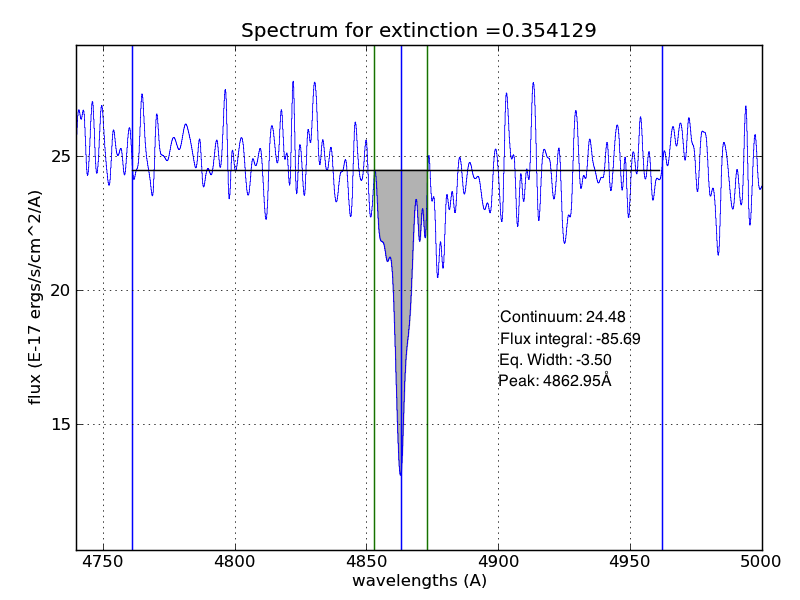
\includegraphics[width=12cm]{../workingexample}\\
Fig. 5. This shows the continuum and equivalent-width estimation. The green lines are each 10$\AA$  away from the central blue line. The blue lines in the extreme left and right are defined at 4761$\AA$ and 4962$\AA$  respectively. \\
\textbf{3. Changing the filters to determine the significance of each color filter in the number of stars	}\\
- Each of the (u-g), (g-r), (r-i) and (i-z) filters was changed individiually from 0.08 to 0.20 in graduations of 0.005, while holding the other three constant at 0.08. 
- It was found that (u-g) and (g-r) were most important for increasing the number of stars; each of these filters was linearly proportional to the number of stars returned by the SQL query, while the (r-i) and (i-z) filters quickly tapered off. \\
\includegraphics[width=6cm]{../varyingug}\includegraphics[width=6cm]{../varyi-z}\\
Fig. 6. On the left, the linear relationship of u-g vs number of stars can be seen, and on the right the nonlinear relationship of r-i vs number of stars can be seen.\\
\textbf{4. Finding relationship between u-g and g-r; triangle.py module}\\
- A scatterplot was made of g-r vs u-g to see if there was a correlation between g-r and u-g. \\
\includegraphics[width=6cm]{../ug&gr2}\\
Fig. 7. A scatter plot of g-r vs u-g; however, it is not clear what the distribution is like, although the there does seem to be a correlation.\\
- The same parameters were taken and with the \href{https://github.com/dfm/triangle.py}{triangle.py module} a corner plot was made, which shows the contours.\\
\includegraphics[width=6cm]{../triangle}\\
Fig. 8. The corner plot, expanded to also include the i-z filter, showing the pairwise distribution of these three filters.\\
\textbf{5. Testing out Linear Discriminant Analysis module for future use}\\
- The LDA module from \href{http://scikit-learn.org/stable/install.html}{scikit-learn} was installed.
- It was tested on the u-g vs g-r plot from above, with the two classes chosen randomly by the objID, so there is no statistical significance in the below plot.\\
\includegraphics[width=6cm]{../LDAtest}\\
Fig. 9. Test application of LDA module to show potential usage. The two classes are color-coded and the boundary line is plotted. The module also allows for Quadratic Discriminant Analysis (not shown).\\
\end{document}